
% this file is called up by thesis.tex
% content in this file will be fed into the main document

%: ----------------------- introduction file header -----------------------
\chapter{Future Work and Conclusions}

% the code below specifies where the figures are stored
\ifpdf
    \graphicspath{{11_future_work_and_conclusions/figures/PNG/}{11_future_work_and_conclusions/figures/PDF/}{11_future_work_and_conclusions/figures/}}
\else
    \graphicspath{{11_future_work_and_conclusions/figures/EPS/}{11_future_work_and_conclusions/figures/}}
\fi

% ----------------------------------------------------------------------
%: ------------------------------- content ----------------------------- 
% ----------------------------------------------------------------------

\begin{figure}
  \centering
  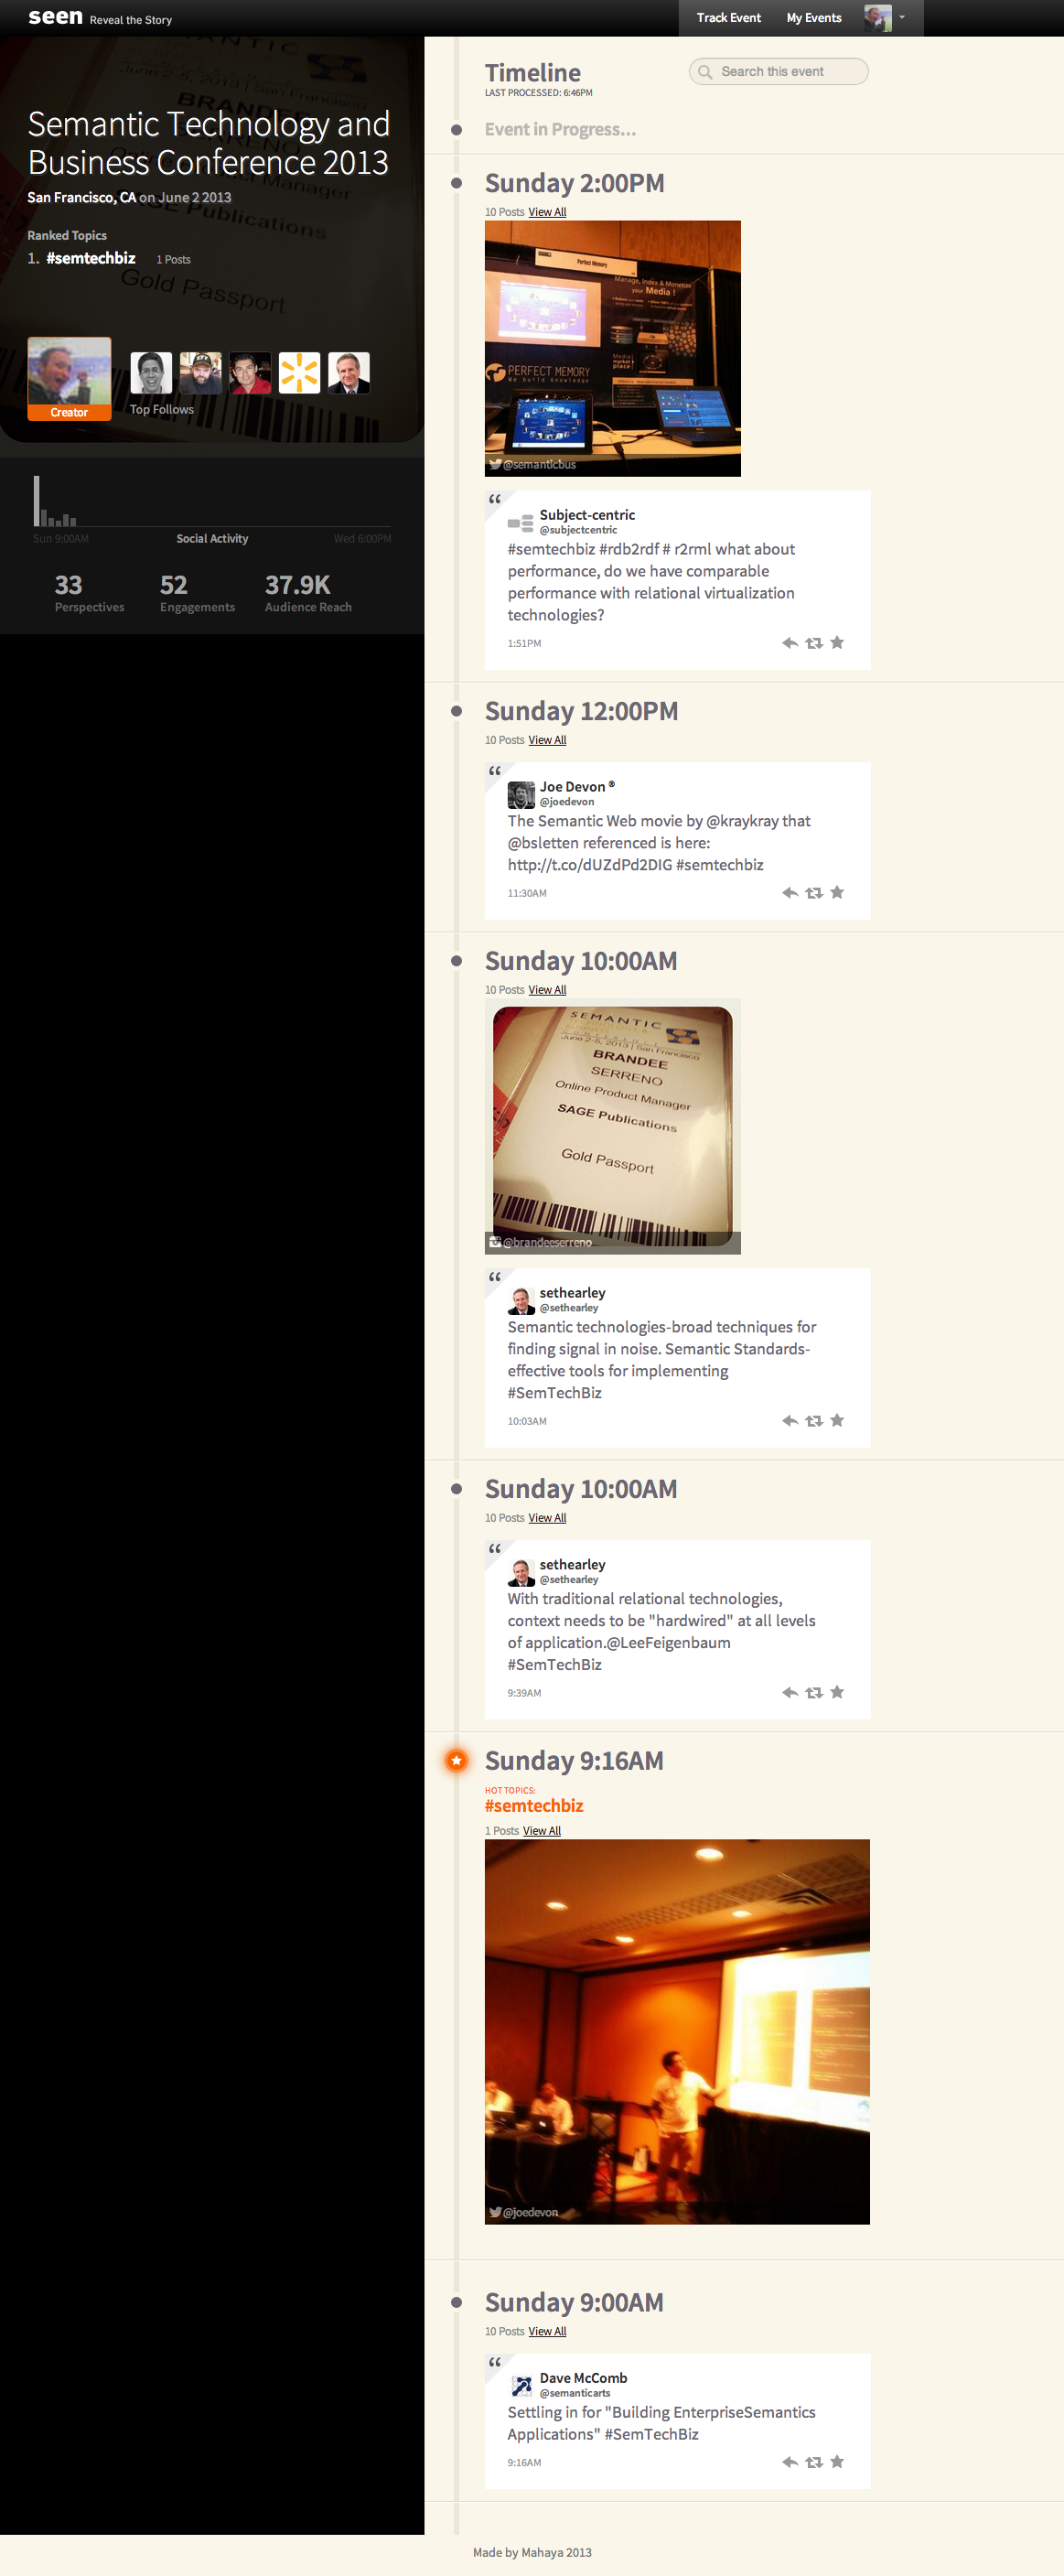
\includegraphics[width=\linewidth]{seen.png}
  \caption{Mahaya's commercial automatic event archiving tool Seen
    (\url{http://mahaya.co/})}
  \label{fig:seen}
\end{figure}

\begin{figure}
  \centering
  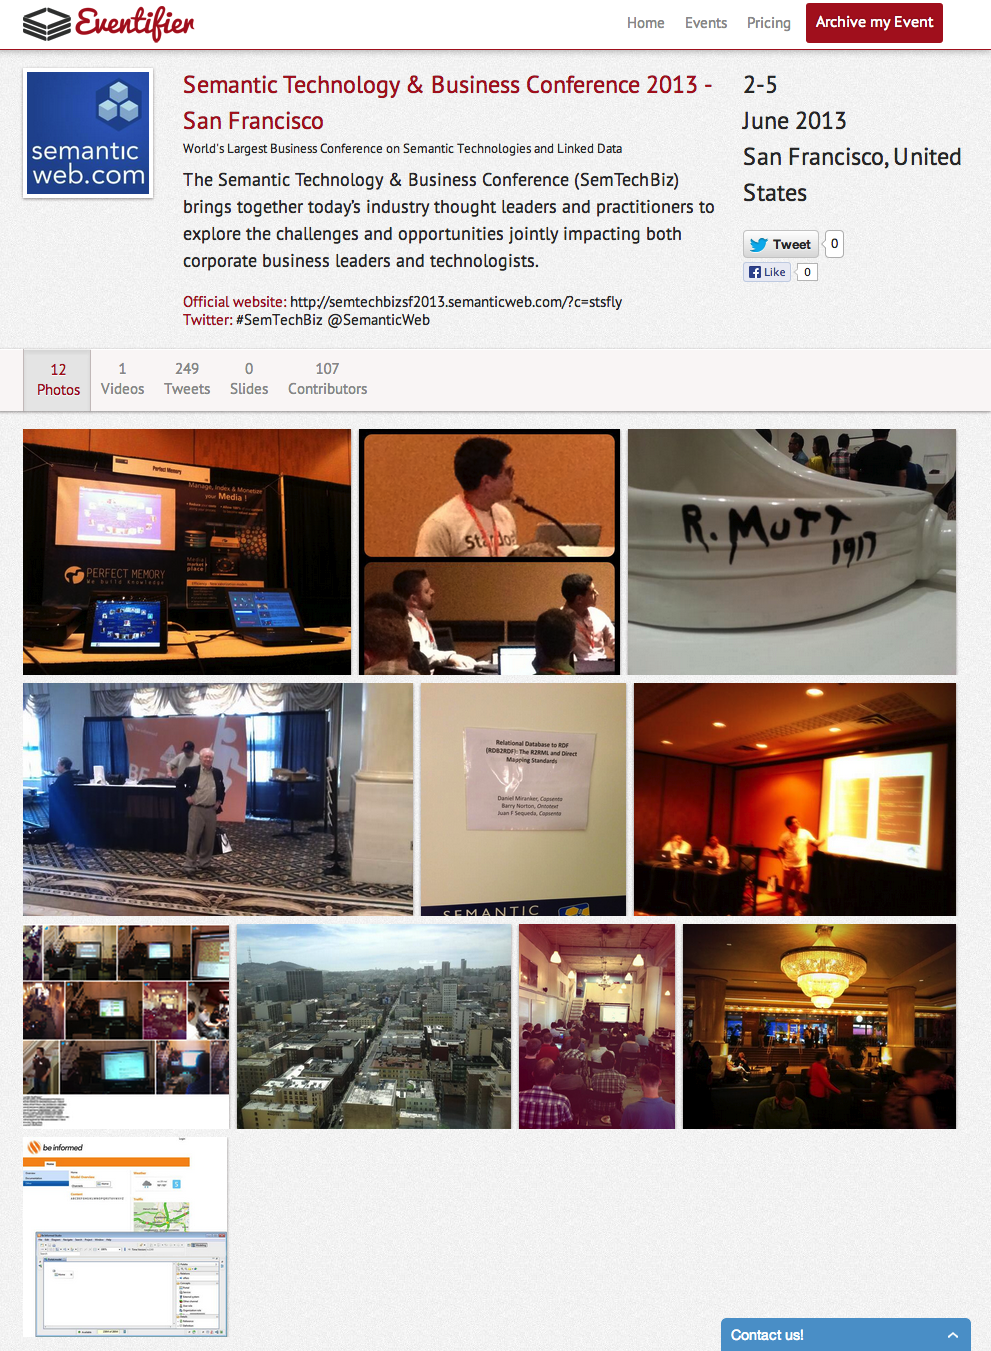
\includegraphics[width=\linewidth]{eventifier.png}
  \caption{The automatic commercial event archiving tool Eventifier
    (\url{http://eventifier.co/})}
  \label{fig:eventifier}
\end{figure}

\begin{figure}
  \centering
  \includegraphics[width=\linewidth]{storify.png}
  \caption{The manual assisted commercial event archiving tool Storify
    (\url{http://storify.com/})}
  \label{fig:storify}
\end{figure}

\begin{figure}
  \centering
  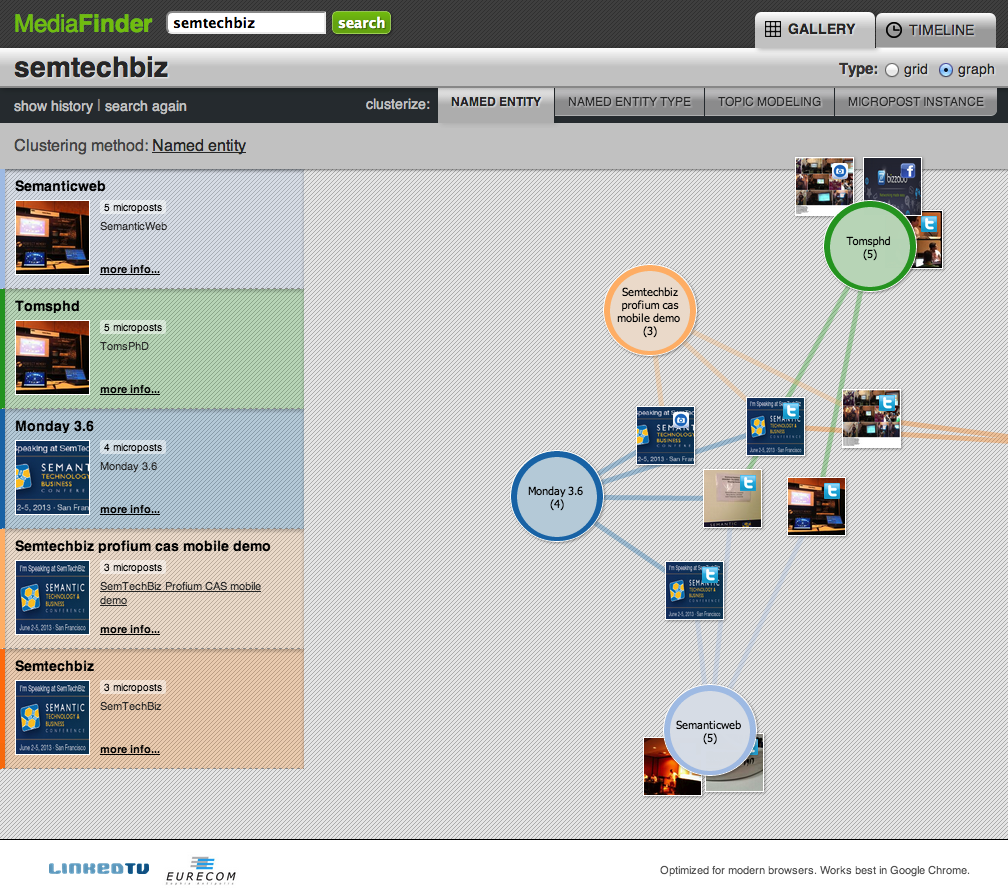
\includegraphics[width=\linewidth]{mediafinder.png}
  \caption{The academic event summarization tool Media Finder}
  \label{fig:mediafinder}
\end{figure}

\begin{figure}
  \centering
  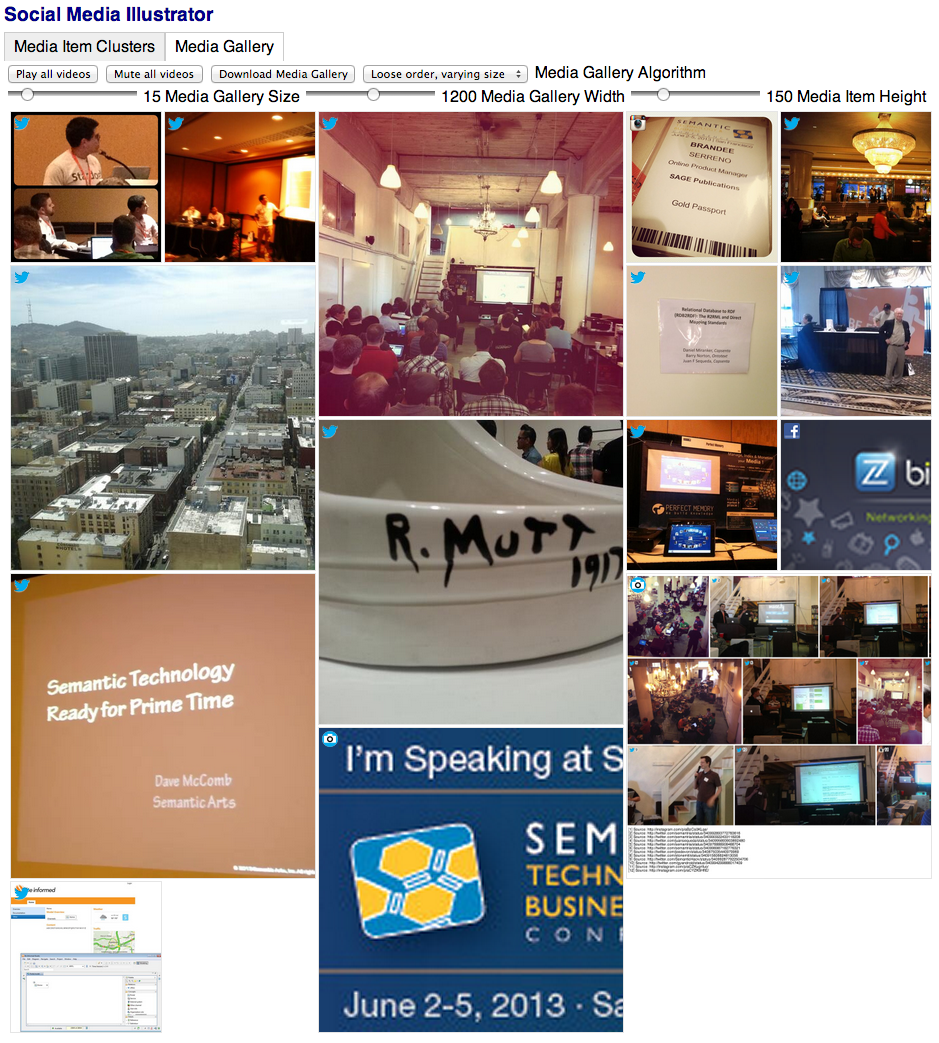
\includegraphics[width=\linewidth]{socialmediaillustrator.png}
  \caption{Our own academic event summarization tool Social Media Illustrator}
  \label{fig:socialmediaillustrator}
\end{figure}

The research fields of event summarization and event archiving
based on social network multimedia data have resulted in 
interesting business creations in recent months.
Albeit similarities to our work exist,
there are still many differences in the details.

\paragraph{Mahaya}
 
The company Mahaya has launched a~beta-version
of a~commercial automatic event archiving tool called Seen,
which, based on manually entered event metadata like event name,
location, and dates, uses a~necessarily provided Twitter hashtag
to create a~complete permanent archive of all event-related tweets,
media items, and slide decks.
Based on term frequency and co-occurrence analyses,
the event is split into subevents
and each subevent's hot topics are tried to be detected.
The application's main data source is Twitter,
links to certain media hosting platforms are followed.
Seen does not deduplicate and cluster
similar media items.

\paragraph{Eventifier}

Eventifier is a~commercial tool that facilitates the automatic permanent archiving of events
in form of event-related photos, videos, tweets, slide decks, 
and event contributors.
Similar to Mahaya's product Seen,
the application's main data source is Twitter.
The manually entered event's official hashtag and potentially existing
official Twitter account serve to encounter event-related content.
Eventifier does not deduplicate and cluster
similar media items.

\paragraph{Storify}

The commercial tool Storify allows for the manual compilation of
event-related media items, articles, and microposts
to generated permanently available stories
that---depending on the level of human curation---%
can efficiently summarize an event.
Storify does not deduplicate and cluster
similar media items.

\paragraph{Media Finder}

Media Finder is an academic non-commercial tool that
has advanced named entity centric clustering capabilities
based on extracted named entities in microposts.
Media items can be clustered by topic, named entity,
named entity type, and micropost instance.
We have contributed the application's media extraction component,
in consequence the covered social networks
are exactly as described in \autoref{cha:media-item-extraction}.

\subsection{Comparison of Tools}

In the previous paragraphs, we have characterized
commercial and non-commercial tools for the tasks
of event summarization and event archiving. 
\autoref{table:toolcomparison} shows how these tools
compare against our own application Social Media Illustrator.
The unique selling point of our application
are its interactive media galleries that together with speech synthesis
as outlined in \autoref{sec:interactivemediagalleries}
allow for truly one of its kind experience when it comes to 
event summary consumption.

\begin{sidewaystable}[h!]
  \centering
  \small
  \begin{tabular}{|l|l|l|l|l|l|}
    \hline
        \backslashbox{\textbf{Property}}{\textbf{Tool}} & \textbf{Seen} & \textbf{Eventifier} & \textbf{Storify} & \textbf{Media Finder} & \textbf{Social Media Illustrator}\\ \hline
      \hline
      \textbf{Data source} & Twitter & Twitter & Multiple & Multiple & Multiple\\
      \textbf{Main task} & Archiving & Archiving & Summarization & Summarization & Summarization\\
      \textbf{Operation mode} & Automatic & Automatic & Manual & Semi-automatic & Semi-automatic\\
      \textbf{Linkable} & Yes & Yes & Yes & Yes & No\\
      \textbf{Downloadable} & No & No & No & No & Yes\\
      \textbf{Customizable} & No & No & Yes & Yes & Yes\\
      \textbf{Interactive} & No & No & No & No & Yes\\
      \textbf{Commercial} & Yes & Yes & Yes & No & No\\
      \hline
    \end{tabular}
    \caption[Comparison of event archiving and summarization tools]{Comparison of commercial and non-commercial event archiving and summarization tools \todo{Check final orientation}}
  \label{table:toolcomparison}
\end{sidewaystable}


Credibility on Storyful.com \url{http://www.ted.com/talks/markham_nolan_how_to_separate_fact_and_fiction_online.html}

\section{Contributions}

\section{Research Directions}





